\chapter{Evaluation \& Testing}\label{ch:Evaluation}
\section{Results}
\subsection{Random Forest: algorithm baseline performance}
In order to set a baseline to compare the results of experiments with under-sampling and oversampling, a Random Forest algorithm was applied to each of the dataset as available after pre-processing. The full script for this experiment can be found in Experiment1.R.\newline
The confusion matrix was obtained from the RandomForestModelling.R script for each dataset and is shown in appendix D1-D10. This data was used to further interpret the results shown in table 5.1.\newline
Table 5.1 shows the results obtained for each dataset. There are three occasions where the performance metrics were not calculated:
\begin{itemize}
    \item The precision value for the Fertility dataset
    \item The F1 value for the Fertility dataset
    \item The F1 value for the modified Heart Attack dataset
\end{itemize}

\begin{table}[!htbp]
\centering
\begin{tabular}{lrrrr}
  \hline
  \rowcolor{LightCyan}
Dataset & Accuracy & Sensitivity & Precision & F1Score \\ 
  \hline
AuSDf & 1.00 & 1.00 & 1.00 & 1.00 \\ 
  BCDf & 0.92 & 0.86 & 0.94 & 0.89 \\ 
  CCDf & 1.00 & 0.90 & 1.00 & 0.95 \\ 
  DiabetesDf & 0.74 & 0.56 & 0.72 & 0.63 \\ 
  FertDf & 0.93 & 0.00 & nd & nd \\ 
  HAPDf & 0.91 & 0.83 & 0.89 & 0.86 \\ 
  LBPDf & 0.82 & 0.90 & 0.84 & 0.87 \\ 
  LiverDf & 0.72 & 0.35 & 0.58 & 0.44 \\ 
  subHAPDf & 0.95 & 0.00 & 0.00 & nd \\ 
  subLBPDf & 0.91 & 0.50 & 1.00 & 0.67 \\ 
   \hline
\end{tabular}
\caption{Performance metrics obtained for Random Forest applied to the chosen datasets}
\end{table}

The data from the confusion matrix output for the Fertility test (Appendix D.5)
show that there were no accurate prediction for the positive class and no inaccurate prediction for the positive class which means the the Precision or Positive predictive value could not be calculated (no division by 0) for this dataset. A lack of Precision value means that the F1 score cannot be calculated as it is obtained by calculated the harmonic mean of Precision and Sensitivity.\newline
This result is partly due to the size of the dataset (only 100 observations and as such there are only 29 observations in the test set). This means that the model will very accurately predict people not suffering infertility but struggles to identify people suffering from infertility.\newline
There is no value for the F1 score of the modified Heart Attack dataset as both the Precision and Sensitivity values are equal to 0 and as such the harmonic mean cannot be calculated (no division by 0).\newline
Table 5.1 also shows that only considering overall accuracy when estimating the performance of an algorithm is misleading. Random Forest returns good to very good accuracy for most of these datasets (accuracy ranges from 0.72 to 1), however, excluding the Autism dataset, the Sensitivity, Precision and F1 score obtained can indicate that although the accuracy is good there is a high chance of the algorithm returning a high number of false positives (low Sensitivity value) or missing out positives (low precision value). \newline
In all cases except the Low Back Pain dataset, there is a majority of cases for the negative class, thus these results are expected. Experimenting with under-sampling and over-sampling of the data is expected to lead to improvement of some of the metrics by reducing the proportion difference between the classes.


\subsection{Under-sampling of the majority class}
\subsubsection{Retaining 75\% of the majority class}
In the first under-sampling experiments 75\% of the majority class was retained. Table 5.2 shows the performance metrics obtained after this operation. Full scripts for this experiments can be found in the Experiment2.R file and the output for the confusion matrix for this experiment are found in Appendix D11-D20.\newline

\begin{table}[ht]
\centering
\begin{tabular}{lrrrr}
  \hline
  \rowcolor{LightCyan}
Dataset & Accuracy & Sensitivity & Precision & F1Score \\ 
  \hline
AuSDf & 1.00 & 1.00 & 1.00 & 1.00 \\ 
  BCDf & 0.88 & 0.91 & 0.81 & 0.86 \\ 
  CCDf & 0.99 & 0.90 & 1.00 & 0.95 \\ 
  DiabetesDf & 0.76 & 0.69 & 0.75 & 0.72 \\ 
  FertDf & 0.91 & 0.33 & 1.00 & 0.50 \\ 
  HAPDf & 0.84 & 0.79 & 0.84 & 0.82 \\ 
  LBPDf & 0.81 & 0.89 & 0.87 & 0.88 \\ 
  LiverDf & 0.62 & 0.47 & 0.50 & 0.49 \\ 
  subHAPDf & 0.98 & 0.00 &  &  \\ 
  subLBPDf & 0.96 & 0.80 & 1.00 & 0.89 \\ 
   \hline
\end{tabular}
\caption{Performance metrics obtained for Random Forest when applied to the chosen datasets after under-sampling the data (75\% majority class retained)}
\end{table}

After 25\% of the majority class was discarded, there was no observable effect on the performance of the algorithm for the Autism dataset. The effects observed on the other datasets varied:
\begin{itemize}
    \item Accuracy increased for the Diabetes, modified Heart Attack and modified Low Back Pain datasets but decreased for the Breast Cancer, Cervical Cancer, Fertility, Heart Attack, Low Back Pain and Liver datasets.
    \item Sensitivity increased for the Breast Cancer, Diabetes and Fertility, Liver and modified Low Back Pain datasets but decreased for the Low Back Pain dataset and remain unchanged for the Cervical Cancer dataset.
    \item Precision decreased for the Breast Cancer and Liver datasets but increased for the Diabetes and Low Pack Pain datasets. It was either unchanged or unavailable for the other datasets.
    \item The F1 score increased for the Diabetes and modified Low Back Pain dataset, but decreased for the Breast Cancer and Heart Attack datasets. For the other datasets it was either unchanged or not available.
\end{itemize}

Excluding Diabetes, modified Heart Attack and modified Low Back Pain datasets, under-sampling resulted in a reduced accuracy, and for most cases increased sensitivity. 


\subsubsection{Retaining 60\% of the majority class}
In the second under-sampling experiments 60\% of the majority class was retained. Table 5.3 shows the performance metrics obtained after this operation. Full scripts for this experiments can be found in the Experiment2.R file and the output for the confusion matrix for this experiment are found in Appendix D21-30.

\begin{table}[ht]
\centering
\begin{tabular}{lrrrr}
  \hline
  \rowcolor{LightCyan}
Dataset & Accuracy & Sensitivity & Precision & F1Score \\ 
  \hline
AuSDf & 1.00 & 1.00 & 1.00 & 1.00 \\ 
  BCDf & 0.98 & 0.95 & 1.00 & 0.97 \\ 
  CCDf & 0.99 & 0.91 & 0.91 & 0.91 \\ 
  DiabetesDf & 0.76 & 0.79 & 0.73 & 0.76 \\ 
  FertDf & 0.59 & 0.00 & 0.00 &  \\ 
  HAPDf & 0.88 & 0.82 & 0.88 & 0.85 \\ 
  LBPDf & 0.82 & 0.95 & 0.85 & 0.90 \\ 
  LiverDf & 0.59 & 0.62 & 0.48 & 0.55 \\ 
  subHAPDf & 0.89 & 0.20 & 1.00 & 0.33 \\ 
  subLBPDf & 0.85 & 0.40 & 1.00 & 0.57 \\ 
   \hline
\end{tabular}
\caption{Performance metrics obtained for Random Forest when applied to the chosen datasets after under-sampling the data (60\% majority class retained)}
\end{table}

Retaining 60\% of the majority class does not appear to affect the performance of the algorithm and the Autism dataset, where all metrics have achieved maximum value.
\begin{itemize}
    \item Accuracy increases in these conditions for the Breast Cancer, Diabetes and Fertility dataset but decreases for the Cervical Cancer, Heart Attack, Liver, modified Heart Attack, modified Low Back Pain datasets.
    \item Sensitivity increases for the Breast Cancer, Cervical Cancer, Diabetes, Low Back Pain, Liver and modified Heart Attack datasets, decreases for the Heart Attack and modified Low back Pain datasets and remains unchanged for the Fertility dataset.
    \item Precision increases for the Breast Cancer, Diabetes, Low Back Pain, modified Heart Attack datasets but decreases for the Cervical Cancer, Heart Attack and Liver datasets.
    \item F1 score increased in Breast Cancer, Diabetes, Low Back Pain, Liver and modified Low Back Pain but decreased for Cervical Cancer and Heart Attack datasets
\end{itemize}

Discarding 40\% of the majority class leads to a decrease in overall accuracy  and an increase in sensitivity (apart from the Heart Attack dataset), the effect on precision is variable and effect on the F1 score values depends on the extent of the variation observed on sensitivity and precision.

\subsubsection{Retaining 40\% of the majority class}
In the third under-sampling experiments 40\% of the majority class was retained. Table 5.4 shows the performance metrics obtained after this operation. Full scripts for this experiments can be found in the Experiment2.R file and the output for the confusion matrix for this experiment are found in Appendix D31-40.

\begin{table}[ht]
\centering
\begin{tabular}{lrrrr}
  \hline
  \rowcolor{LightCyan}
Dataset & Accuracy & Sensitivity & Precision & F1Score \\ 
  \hline
AuSDf & 1.00 & 1.00 & 1.00 & 1.00 \\ 
  BCDf & 0.95 & 0.95 & 0.97 & 0.96 \\ 
  CCDf & 0.97 & 1.00 & 0.81 & 0.90 \\ 
  DiabetesDf & 0.69 & 0.83 & 0.70 & 0.76 \\ 
  FertDf & 0.82 & 0.00 &  &  \\ 
  HAPDf & 0.79 & 0.89 & 0.76 & 0.82 \\ 
  LBPDf & 0.82 & 1.00 & 0.82 & 0.90 \\ 
  LiverDf & 0.65 & 0.74 & 0.61 & 0.67 \\ 
  subHAPDf & 0.92 & 0.00 & 0.00 &  \\ 
  subLBPDf & 1.00 & 1.00 & 1.00 & 1.00 \\ 
   \hline
\end{tabular}
\caption{Performance metrics obtained for Random Forest when applied to the chosen datasets after under-sampling the data (40\% majority class retained)}
\end{table}

The performance of Random Forest on the Autism dataset after under-sampling to that extent is not affected at all. Although 60\%of the majority class has been discarded, all the metrics have achieved maximum value.
\begin{itemize}
    \item Accuracy decreases for the Cervical Cancer, Diabetes, Fertility, Heart Attack, Low Back Pain, Liver and modified Heart Attack datasets but increased for the modified Low Back Pain and Breast Cancer datasets
    \item Sensitivity increased for all datasets except Fertility and modified Heart Attack where it was unchanged.
    \item Precision was increased for Breast Cancer and Liver datasets but decreased for all other datasets where it was calculated.
    \item F1 score increased for Breast Cancer, Diabetes, Low Back Pain, Liver and modified Low Back Pain datasets but decreased for the Cervical Cancer and Heart Attack dataset.
\end{itemize}

The variations between the performance metrics obtained for each of the under-sampling conditions were calculated compared to the established baseline in experiment 1.\newline
The variations for Accuracy, Sensitivity, Precision and Accuracy are shown in the Appendix tables D1-D4.
These values were used to create graphs to represent the variations for each metrics in the different conditions and for the different datasets.\newline


\begin{figure}[!htbp]
    \centering
    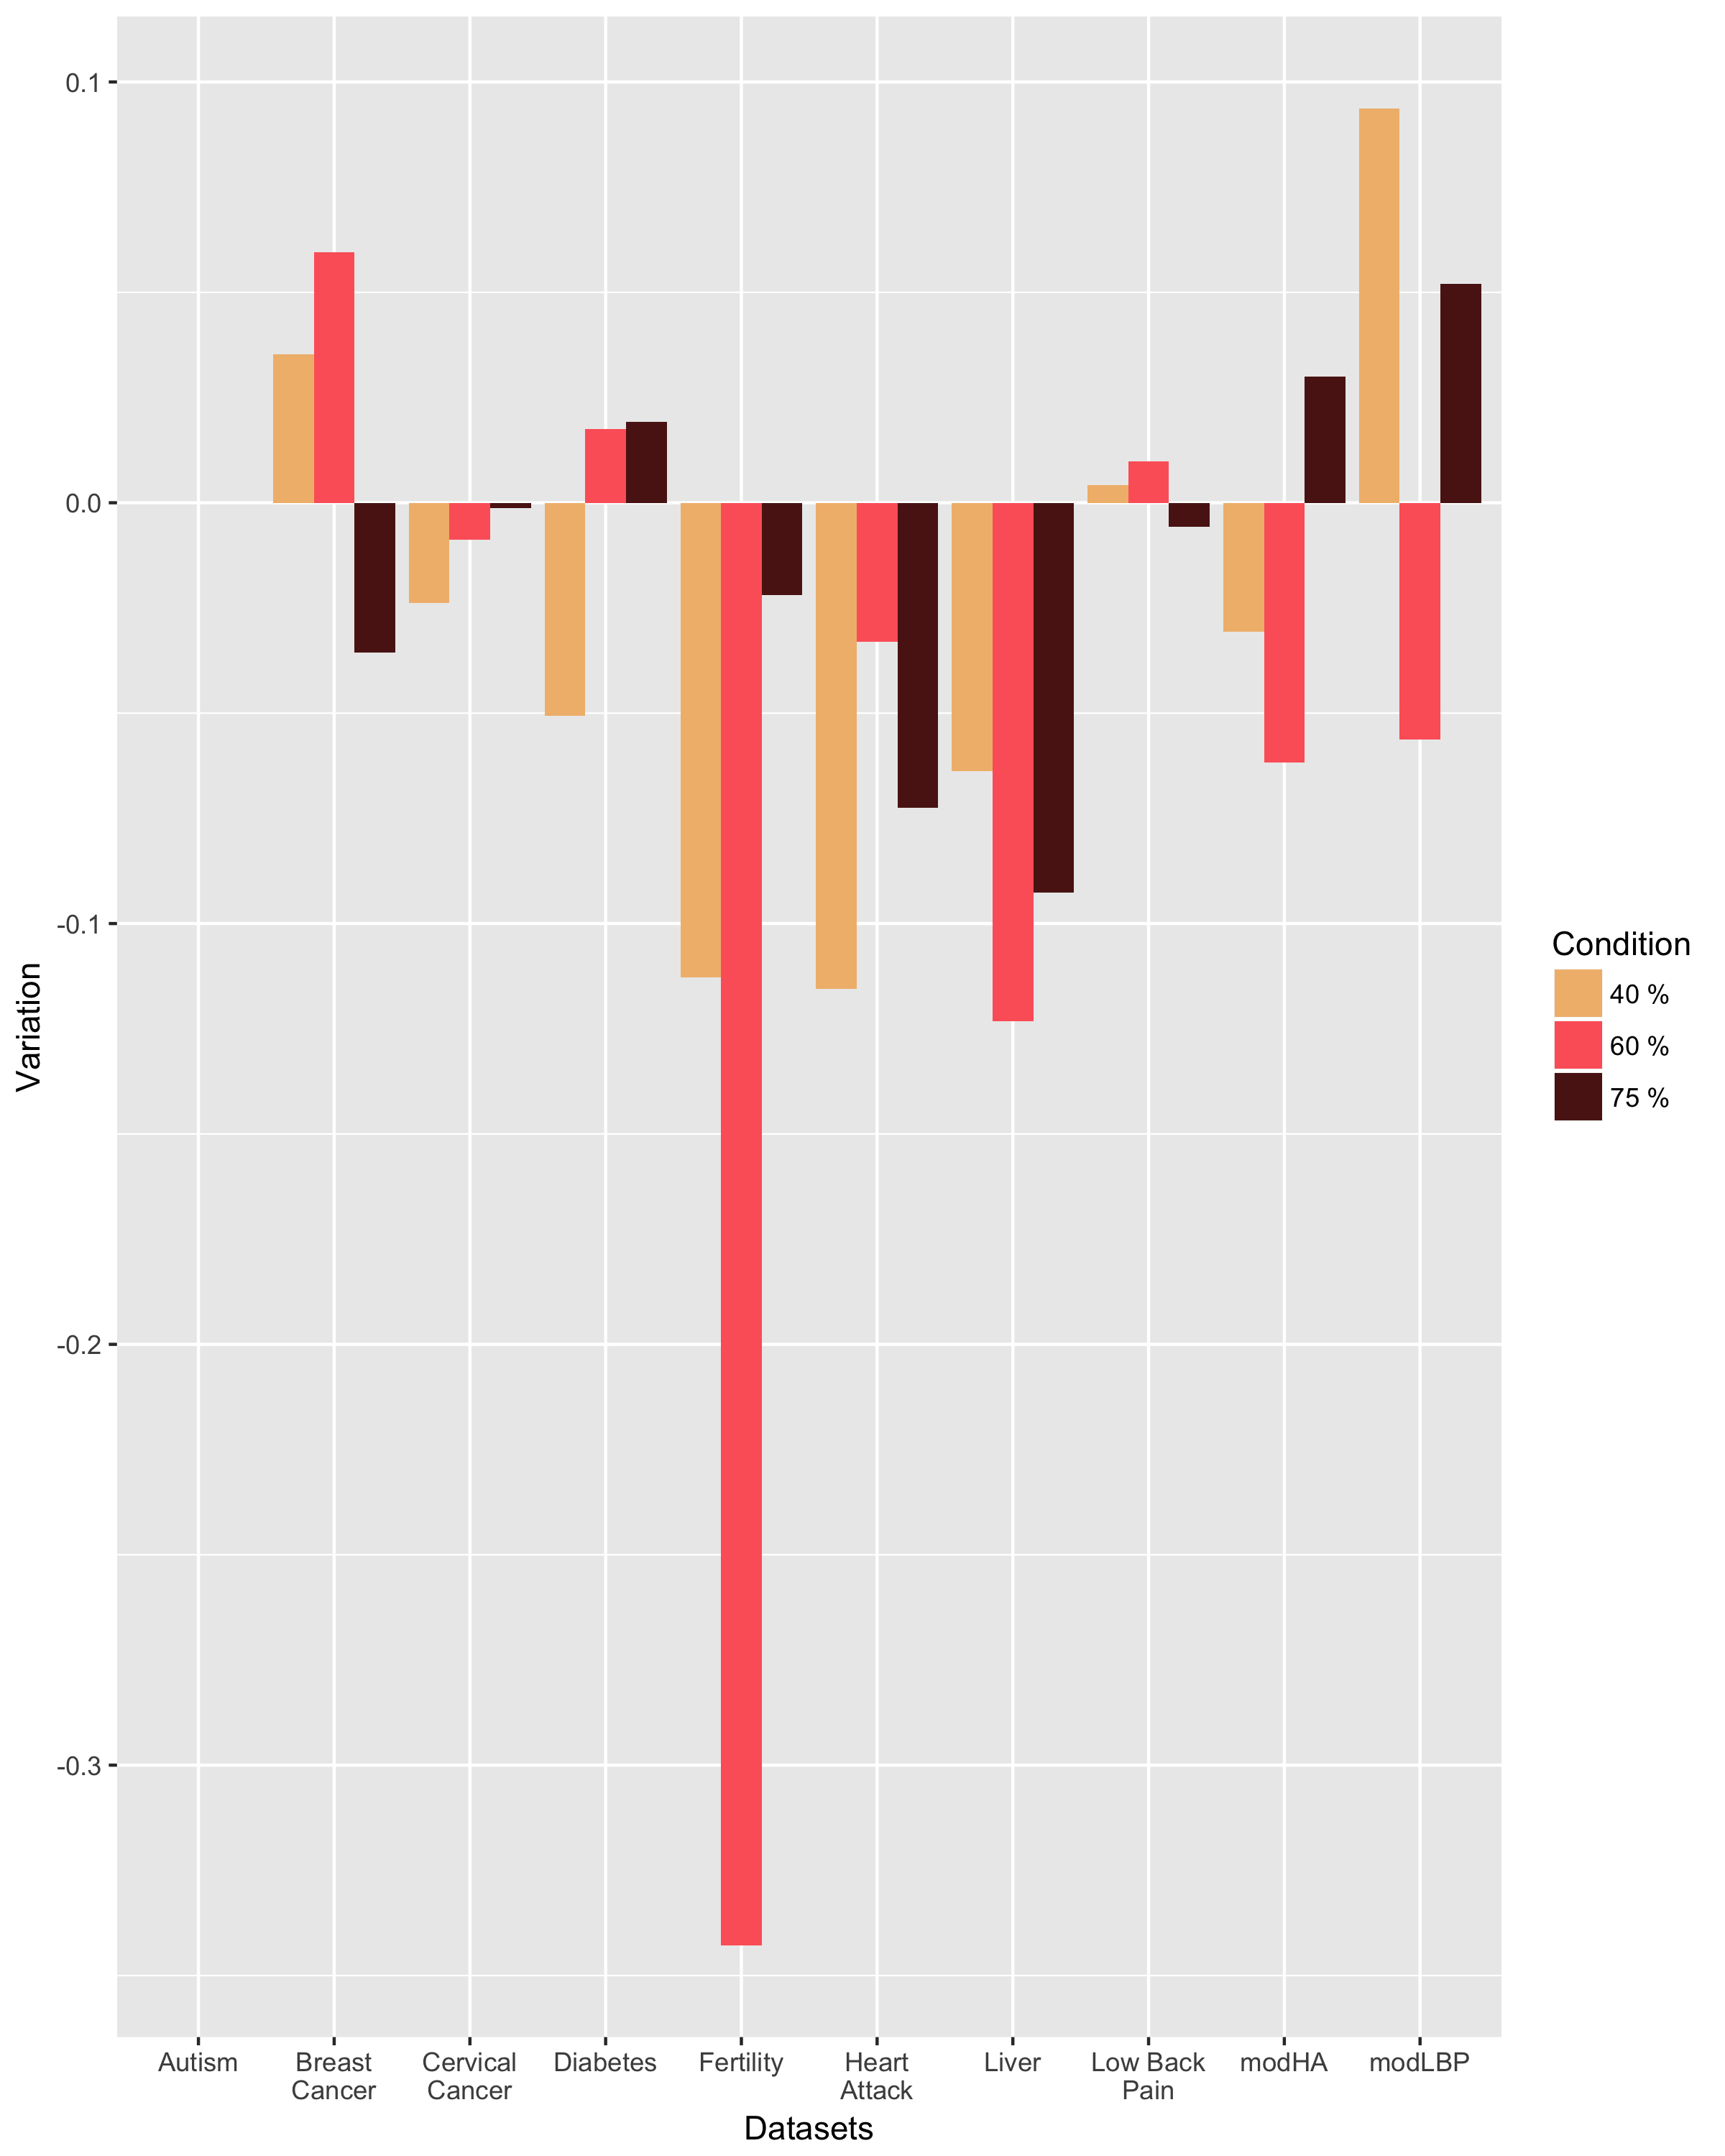
\includegraphics[width=0.9\textwidth]{ThesisTemplate/usingLatex/chapter5Images/AccuVariationUnderBySets.png}
    \caption{Variation of the accuracy value for the three under-sampling conditions compared to the baseline established in Experiment 1 for all studied datasets.}
    \label{fig:my_label}
\end{figure}

Figure 5.1 shows the variations in accuracy observed when 75\%, 60\% and 40\% of the majority class was retained.
Overall the effect is that of a decrease in accuracy when under-sampling of the  majority class is applied, though the effect is slight (less than 0.15 variation for most datasets, except for the Diabetes dataset where the accuracy is greatly affected when under-sampling occurs).\newline



\begin{figure}[!htbp]
    \centering
    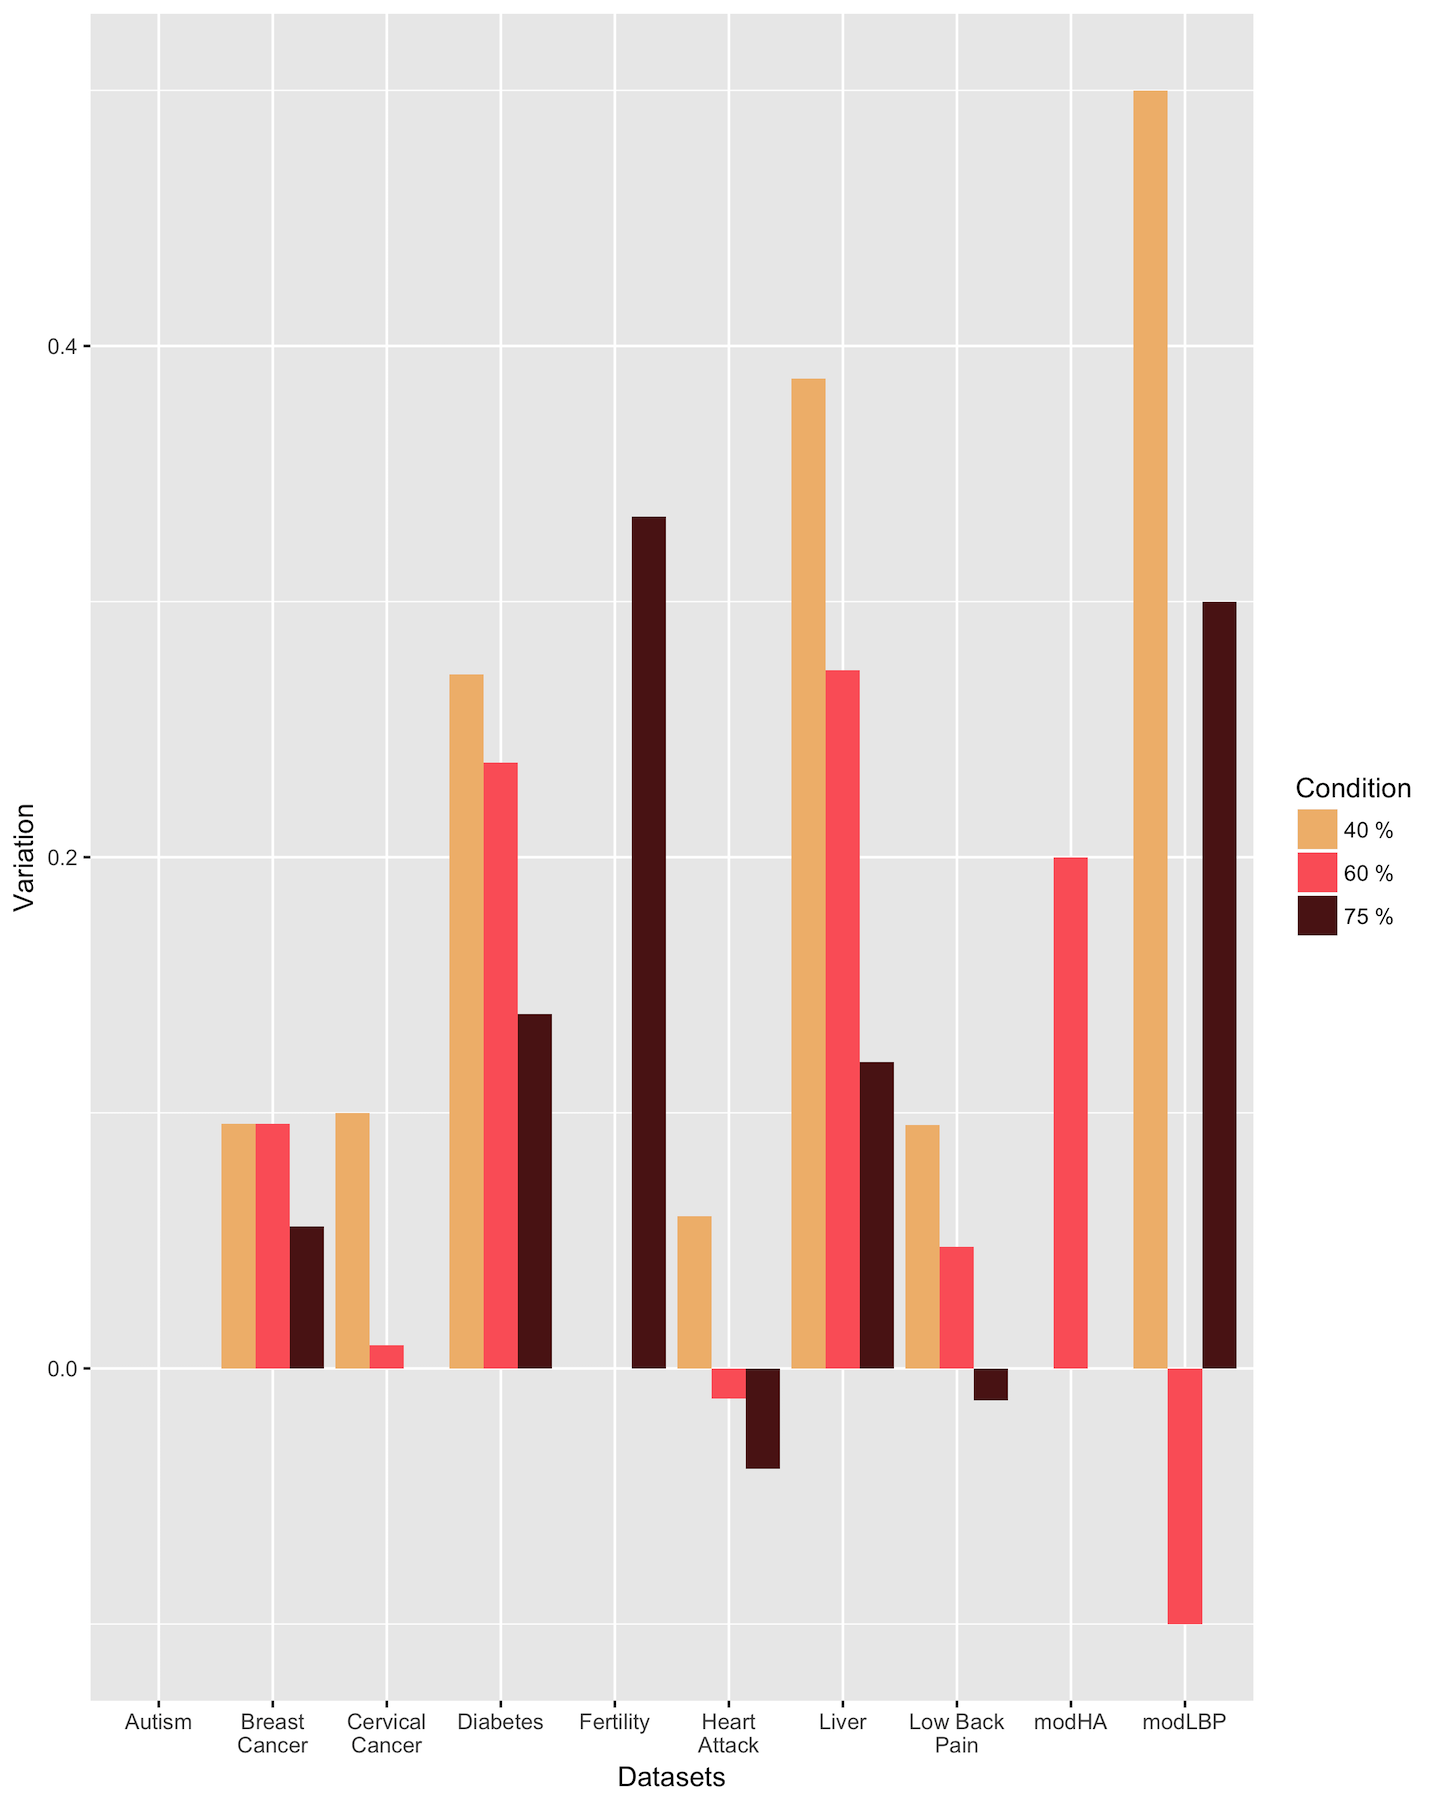
\includegraphics[width=0.9\textwidth]{ThesisTemplate/usingLatex/chapter5Images/SensiVariationUnderBySets.png}
    \caption{Variation of the sensitivity value for the three under-sampling conditions compared to the baseline established in Experiment 1 for all studied datasets.}
    \label{fig:my_label}
\end{figure}
Figure 5.2 shows the variations in sensitivity observed when   75\%, 60\% and 40\% of the majority class was retained. The overall effect is that sensitivity increases when under-sampling is applied; The trend is that the more of the majority class has been discarded, the more the sensitivity increases, the highest observed increase is 0.4.\newline



\begin{figure}[!htbp]
    \centering
    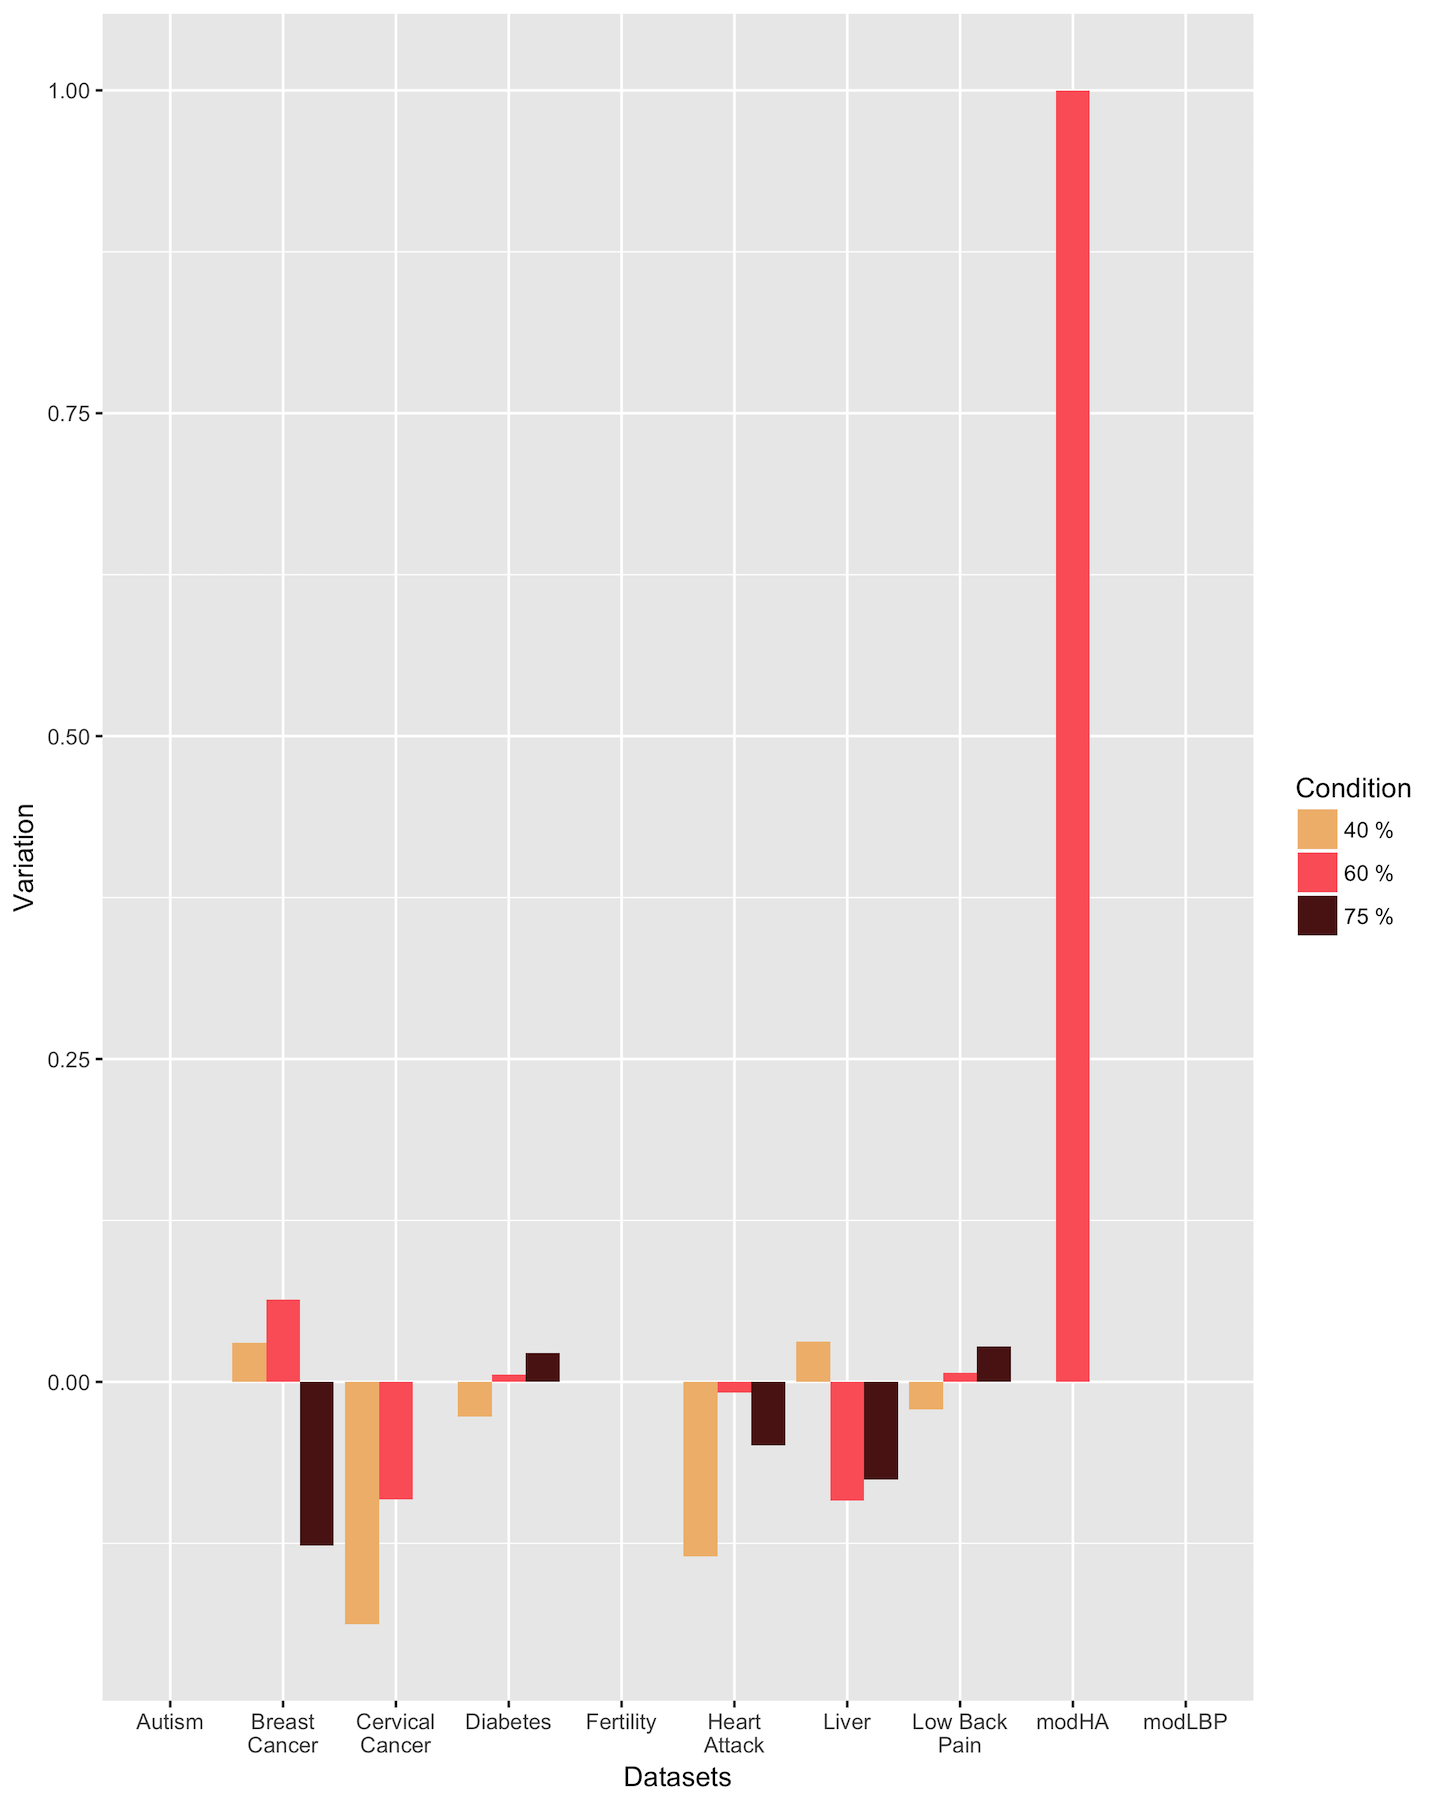
\includegraphics[width=0.9\textwidth]{ThesisTemplate/usingLatex/chapter5Images/PreciVariationUnderBySets.png}
    \caption{Variation of the precision value for the three under-sampling conditions compared to the baseline established in Experiment 1 for all studied datasets.}
    \label{fig:my_label}
\end{figure}

Figure 5.3 shows the variations in precision observed when 75\%, 60\% and 40\% of the majority class was retained. In general, precision is reduced by under-sampling, particularly if the proportion of the majority class to be discarded is large, though the effect remains light (maximum reduction is 0.19) In one case (modified Heart Attack dataset), the precision value is greatly increase when 60\% of the majority class is retained, though that effect is not consistent with what is observed on the other datasets.\newline

\begin{figure}[!htbp]
    \centering
    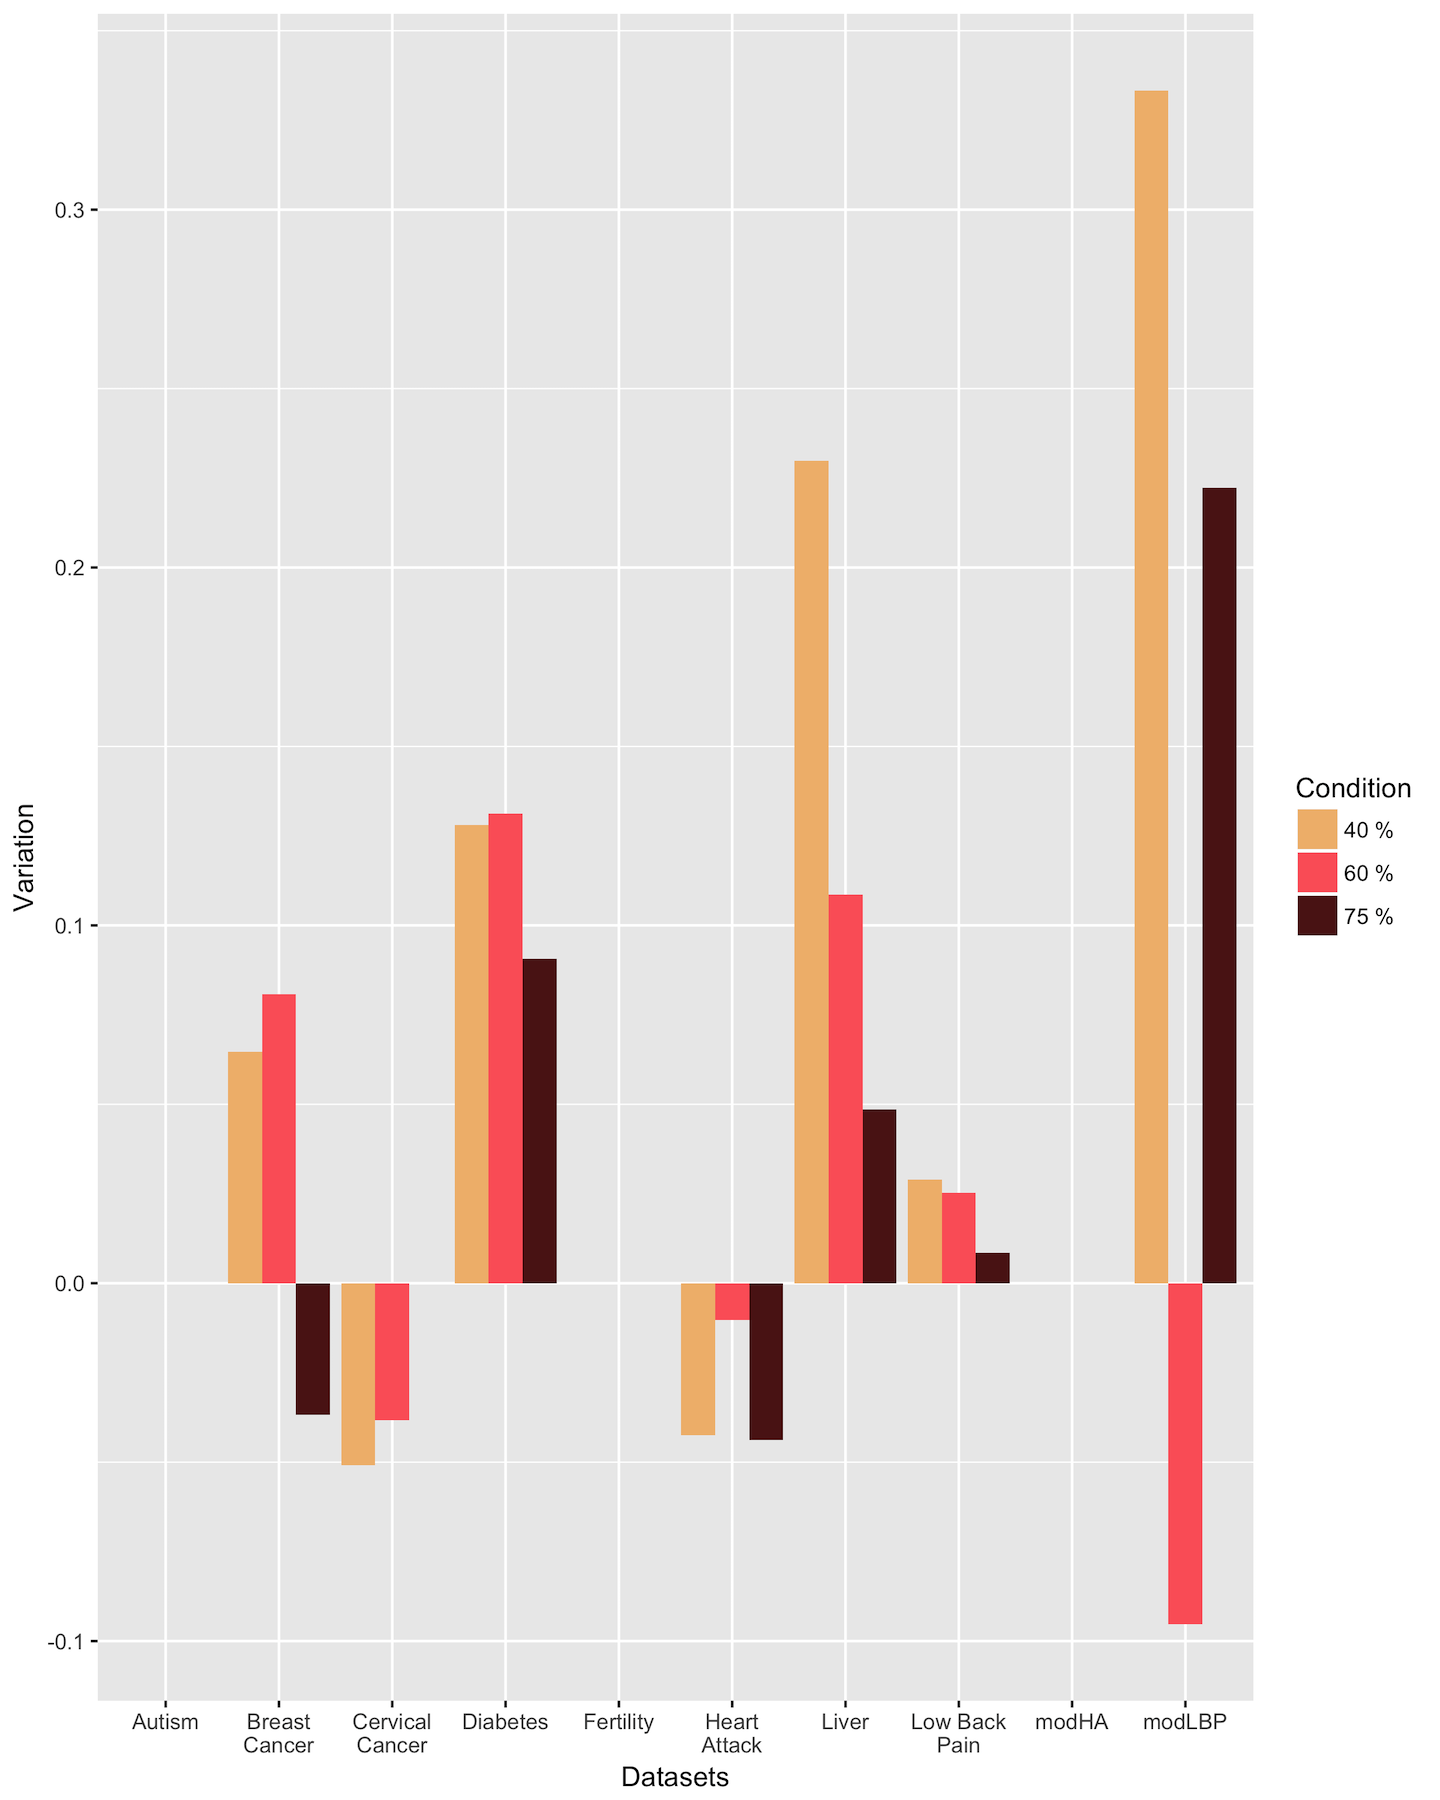
\includegraphics[width=0.9\textwidth]{ThesisTemplate/usingLatex/chapter5Images/F1VariationUnderBySets.png}
    \caption{Variation of the F1 score value for the three under-sampling conditions compared to the baseline established in Experiment 1 for all studied datasets.}
    \label{fig:my_label}
\end{figure}

Figure 5.4 shows the variations in F1 score observed when 75\%, 60\% and 40\% of the majority class was retained. In general the F1 score increases with the increased proportion of discarded majority class. The F1 score is partly dependent on both precision and sensitivity, but as previously discussed sensitivity tends to increase when the proportion of majority class discarded increases while precision decreases when the proportion of majority class discarded increases but to a lesser extent; thus the overall effect on the F1 score is that it increases as the proportion of majority class discarded increases.\newline



\subsection{Over-sampling the minority class (SMOTE)}
Over-sampling was carried out using the smote() function of R (see script Experiment3.R).\newline
The table below shows the new class distribution of the training sets after the smote() function was applied as described in section 4.3.2.\newline

\begin{table}[!htbp]
\centering
\begin{tabular}{lrrrr}
  \hline
  \rowcolor{LightCyan}
Dataset & MajorityClass & MinorityClass & NewMajorityClass & NewMinorityClass \\ 
  \hline
AuSDf [1] & 353 & 140 & 280 & 280 \\ 
  BCDf [1] & 258 & 143 & 286 & 286 \\ 
  CCDf [1] & 573 &  29 &  58 &  58 \\ 
  DiabetesDf [1] & 362 & 178 & 356 & 356 \\ 
  HAPDf [1] & 131 &  76 & 152 & 152 \\ 
  LBPDf [1] &  71 & 147 & 142 & 142 \\ 
  LiverDf [1]& 297 & 113 & 226 & 226 \\ 
   \hline
subHAPDf [2]& 134 &   7 & 112 &  63 \\ 
  subLBPDf [2] &  72 &  10 & 160 &  90 \\ 
  \hline
FertDf [3] &  61 &  10 & 120 &  70 \\ 
   \hline
\end{tabular}
\caption{Class distribution of the training sets before and after smote() has been applied with the parameters [1]:perc.under =100, perc.over =200, k=4, [2]: perc.under =200, perc.over = 800, k=4, [3]: perc.under =200, perc.over = 600, k=4}
\end{table}

With these parameters, a new class distribution was achieved of 1:1 ratio majority:minority for the the Autism, Breast Cancer, Cervical Cancer, Diabetes, Heart Attack, Low Back Pain and Liver datasets. The new ratio observed for modified Heart Attack, modified Low Back Pain and Fertility is 1.7:1. \newline
Table 5.6 shows the results obtained for the performance metrics for Random Forest after SMOTE was carried out.\newline
As previously noted, the results obtained for the Autism dataset are unchanged when SMOTE has been applied to the dataset. For the other 6 datasets, a decrease in Accuracy can be noted for Cervical Cancer and Liver datasets but it is increased for Breast Cancer and unchanged for the others.
Sensitivity is increased for Breast Cancer, Cervical Cancer, Diabetes and Heart Attack datasets but decreased for Low Back Pain and Liver datasets. Precision is increased for Breast Cancer, Cervical Cancer, Low back Pain and Liver datasets but decreased for Diabetes and Heart Attack. Finally the F1 score is increased for Breast Cancer, Diabetes and Liver. It is unchanged for Heart Attack and it decreases for Cervical Cancer and Low Back Pain.\newline

\begin{table}[!htbp]
\centering
\begin{tabular}{lrrrr}
  \hline
  \rowcolor{LightCyan}
Dataset & Accuracy & Sensitivity & Precision & F1Score \\ 
  \hline
AuSDf & 1 & 1.00 & 1.00 & 1.00 \\ 
  BCDf & 0.9464 & 0.96 & 0.92 & 0.94 \\ 
  CCDf & 0.9688 & 1.00 & 0.56 & 0.71 \\ 
  DiabetesDf & 0.7412 & 0.72 & 0.66 & 0.69 \\ 
  HAPDf & 0.8966 & 0.90 & 0.82 & 0.86 \\ 
  LBPDf & 0.8152 & 0.81 & 0.91 & 0.86 \\ 
  LiverDf & 0.6821 & 0.85 & 0.49 & 0.63 \\ 
  subHAPDf & 0.9474 & 0.67 & 0.50 & 0.57 \\ 
  subLBPDf & 0.7500 & 0.50 & 0.25 & 0.33 \\ 
  FertDf & 0.7241 & 0.50 & 0.12 & 0.20 \\ 
   \hline
\end{tabular}
\caption{Performance metrics obtained after smote has been applied to the training sets}
\end{table}

 The smote() function was applied to the datasets Fertility, modified Heart Attack and modified Low Back Pain with different parameters (see Chapter 4.3.2). These datasets already contain a low number of observations,  particularly in the minority class so the the training test contained even less observations in the minority class. If the parameters used for the other datasets are applied to Fertility, modified Heart Attack and modified Low Back Pain, not enough majority class points are retained compared to the newly generated minority class observations, thus leading to a large amount of data loss.\newline
The new class distribution obtained for these datasets after SMOTE was applied is shown in table 5.5.\newline
The results obtained after SMOTE was applied to the modified Heart Attack, Low Back Pain and Fertility datasets are shown in table 5.6.\newline
For the modified Heart Attack and modified Low Back Pain datasets, the Accuracy was decreased in both cases. Sensitivity was increased for modified Heart Attack but unchanged for the modified Low Back Pain. Precision was increased for modified Heart Attack but decreased for modified Low Back Pain and the F1 score increased in both cases.\newline
In this case of the Fertility dataset, although the overall accuracy of the algorithm was reduced, the sensitivity was increased and both precision and F1 score were given a value (when Random Forest is applied to the dataset without prior modification both precision and F1 returned a non-value).\newline
Table D.5 in the Appendix shows the variations observed for each of the metrics when compared to the baseline established in Experiment 1 and they are represented on figure 5.5.\newline

\begin{figure}[!htbp]
    \centering
    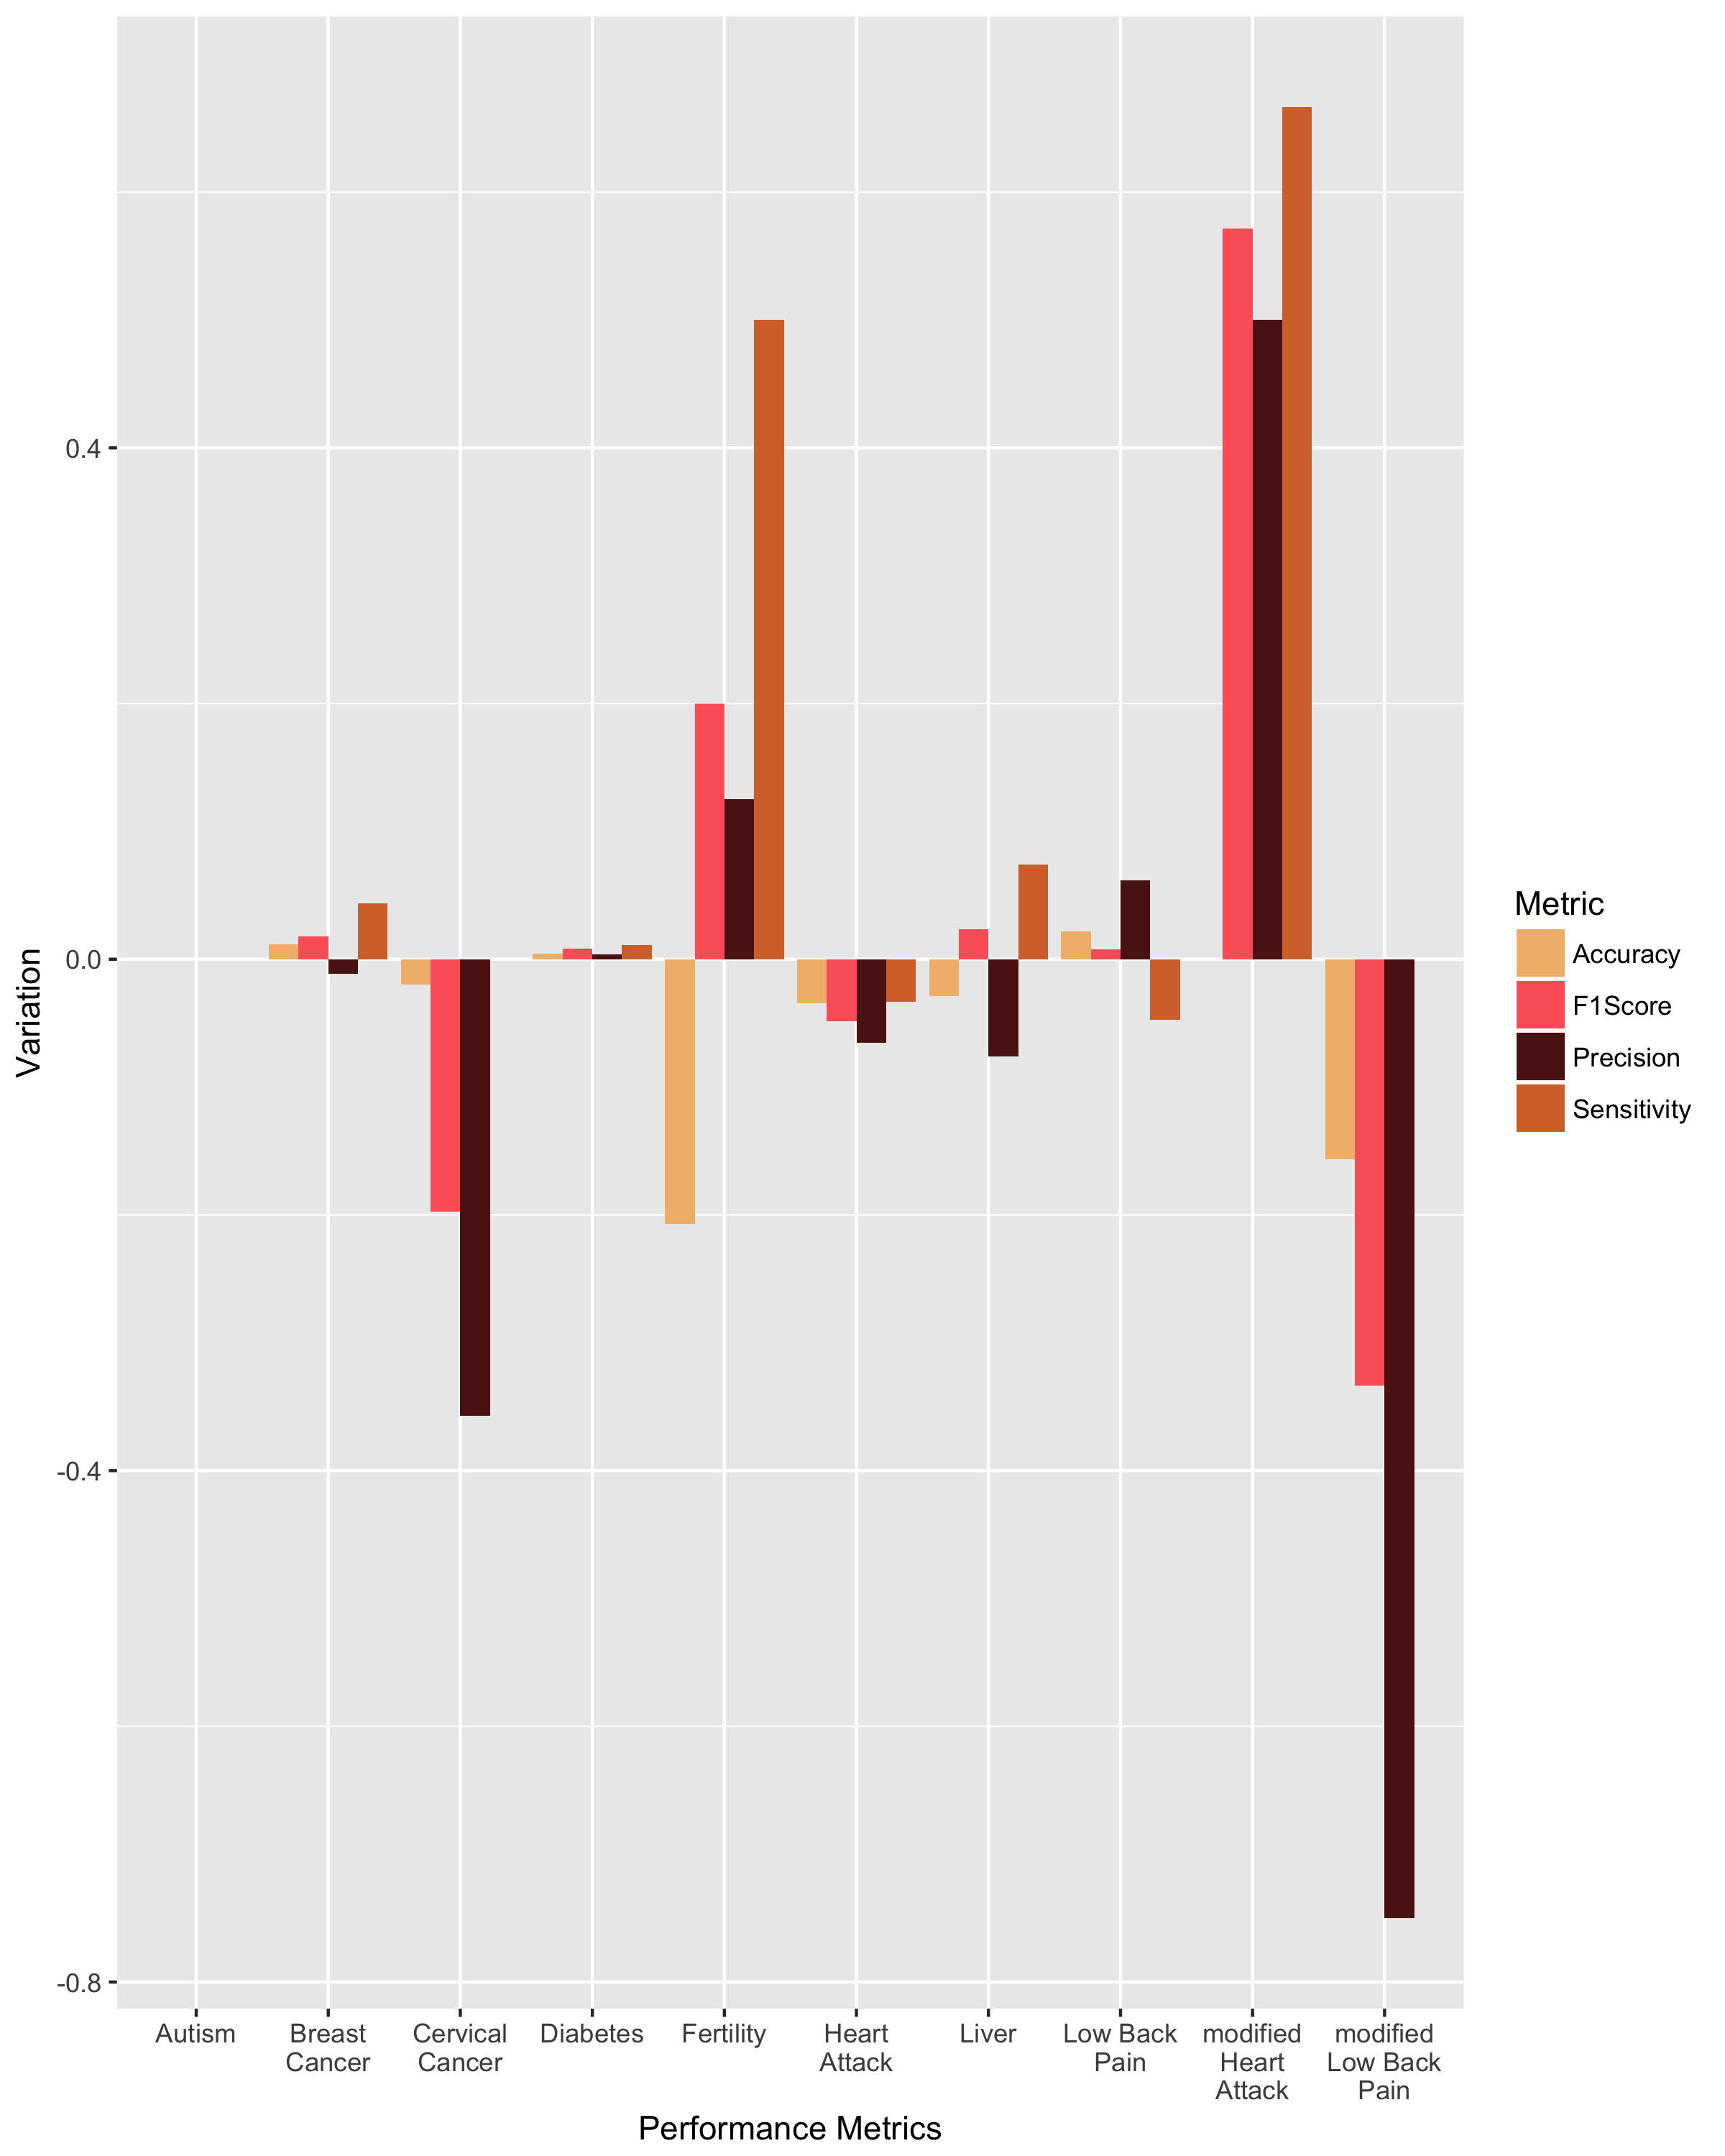
\includegraphics[width=0.9\textwidth]{ThesisTemplate/usingLatex/chapter5Images/OverVariations.png}
    \caption{Observed variations for all measured metrics after SMOTE compared to the baseline established in Experiment 1 for all studied datasets.}
    \label{fig:my_label}
\end{figure}






\section{Discussion}
\subsection{Under-sampling}
The mean variation for each performance metric was calculated for all three different conditions of under-sampling in order to establish which situation on average would offer the best outcome. Best outcome was defined as minimum reduction in accuracy while sensitivity, precision and F1 score showed improvement.\newline
In the context of medical diagnosis an increased sensitivity (\textit{i.e} reduced number of false negatives) would mean a better ability to find patients suffering from a given condition.\newline Precision on the other hand reflects the ability to discriminate for false positive (an increased value for precision means that the algorithms picks out less false positive). When discussing the impact of these values for a medical diagnostic tool, it is important to consider what they mean practically. Ideally, a algorithm would have both high precision and high sensitivity so that few "sick" patients would be missed and few "healthy" patients would be misdiagnosed as sick.\newline
With these considerations in mind, although the under-sampling which eliminated 60\% of the majority class yielded the highest improvement in Sensitivity it also saw the biggest reduction in Precision and the second biggest reduction in Accuracy. Discarding 40\% of the majority class not only increased Sensitivity but also Precision, though the reduction in Accuracy was the highest of the three situation.\newline
Finally, preserving 75\% of the majority class produced the second largest increase in Sensitivity, and decreased Precision less than when 60\% of the majority class was discarded, while decreasing Accuracy the least.\newline
In terms of real-life consequences, it would be less problematic for an individual to be told that they may suffer a condition and require more test to confirm diagnostic (even if they are in fact confirmed to be healthy), than to be given a clean bill of health when they should have been identified as having a particular condition. As such, Sensitivity should be given more importance than Precision (though precision should still be viewed as important, particularly if computer-aided diagnostic is to help deliver more efficient healthcare) and Accuracy should remain high overall. This would suggest that best approach to improving algorithm performance over all the datasets used in this experiment would be to under-sample by discarding 25\% of the majority class only. This is an average outcome and as seen in the detailed graphs, for some datasets, discarding large amount of the majority class was necessary in order to correctly identify the sick patients at all (\textit{e.g.} Fertility dataset). \newline


\begin{table}[!htbp]
    \centering
    \begin{tabular}{p{0.8cm}p{0.8cm}p{0.8cm}p{0.8cm}p{0.8cm}p{0.8cm}p{0.8cm}p{0.8cm}p{0.8cm}p{0.8cm}p{0.8cm}p{0.8cm}}
        \hline
        \rowcolor{LightCyan}
          \multicolumn{3}{c}{Accuracy}& \multicolumn{3}{c}{Sensitivity} & \multicolumn{3}{c}{Precision} & \multicolumn{3}{c}{F1Score}  \\
          \hline
         40\% Maj & 60\% Maj & 75\% Maj & 40\% Maj & 60\% Maj & 75\% Maj & 40\% Maj & 60\% Maj & 75\% Maj & 40\% Maj & 60\% Maj & 75\% Maj \\
         -0.029&-0.060&-0.014&+0.168&+0.083&+0.100& -0.039&+0.111& -0.029&+0.098&+0.029&+0.041
    \end{tabular}
    \caption{Mean of the variations observed on the Accuracy, Precision, Sensitivity and F1 score across all datasets for each under-sampling situation}
    \label{tab:my_label}
\end{table}    	
    	
    	

Statistical analysis was carried out on the values obtained from Experiments 1 and 2. An independent t-test was carried out using the software SSPS to evaluate the significance of the variations for each metrics between the baseline (no under-sampling) and each under-sampling condition.\newline
The output files from SSPS can be found in the github repository and in the appendix. Table 5.5. shows the 2-tail t-test sigma values obtained for each test. All tests were carried out with and without the values for the Autism dataset as these remained unchanged in all experiments and may have affected the results of the t-test.\newline
None of the sigma values are inferior to 0.05, which means that the observed differences are not significant. It is however worth noting that the samples for each test is small as only 10 datasets were analysed and in some cases the precision or F1 score values were not available, further reducing the number of available cases to be considered. A more extensive analysis with a larger number of datasets could potentially yield statistically significant results.\newline

\begin{table}[!htbp]
\centering
\begin{tabular}{*9c}
  \hline
  \rowcolor{LightCyan}
Condition &\multicolumn{2}{c}{Accuracy} &\multicolumn{2}{c}{Sensitivity} &\multicolumn{2}{c}{Precision}&\multicolumn{2}{c}{F1.Score}\\
  \hline
           & [A] & [B] & [A] & [B] & [A] & [B] & [A] & [B] \\
Under 40  &0.608& 0.581& 0.395 & 0.375 & 0.820 & 0.815 & 0.297 & 0.255 \\ 
  Under 60 &0.353& 0.318& 0.649 & 0.628 & 0.941 & 0.925 & 0.789 & 0.800 \\ 
  Under 75 &0.797&0.783 & 0.570 & 0.544 & 0.476 & 0.476 & 0.999 & 0.967 \\ 
   \hline
\end{tabular}
\caption{2-tail t-test sigma values for independent t-test carried out on the results obtained for accuracy, sensitivity, precision and F1 score for each of the datasets. [A] Values obtained while keeping the results for the Autism dataset, [B] values obtained while removing the results obtained for the Autism dataset as they were unchanged in any of the conditions.}
\end{table}
 

\section{Conclusions}

The main conclusions for this chapter.


